\chapter{Project Description 
\index{Chapter!Project Description}
\index{Project Description}
\label{Project Description}}
\begin{figure}[H]
  \centering
  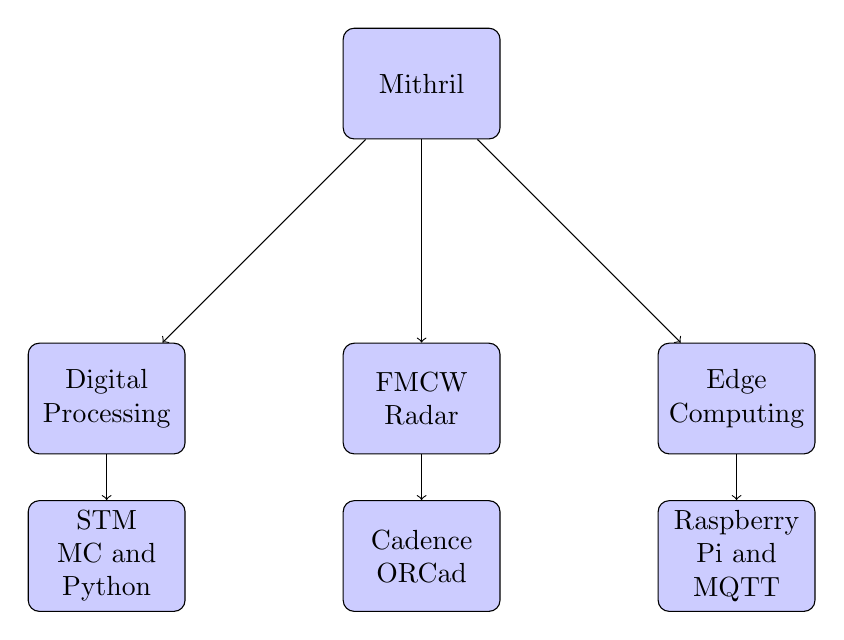
\begin{tikzpicture}[node distance = 2cm, auto]
      % Define block styles
      \tikzstyle{block} = [rectangle, draw, fill=blue!20, 
          text width=5em, text centered, rounded corners, minimum height=4em]
      \tikzstyle{line} = [draw, ->]
  
      % Place nodes
      \node [block] (mithril) {Mithril};
      \node [block, below of=mithril, node distance=4cm] (radar) {FMCW Radar};
      \node [block, left of=radar, node distance=4cm] (processing) {Digital Processing};
      \node [block, right of=radar, node distance=4cm] (networking) {Edge Computing};
      \node [block, below of=processing, node distance=2cm] (STM) {STM MC and Python};
      \node [block, below of=radar, node distance=2cm] (ORCad) {Cadence ORCad};
      \node [block, below of=networking, node distance=2cm] (pi) {Raspberry Pi and MQTT};
      % Draw edges
      \path [line] (mithril) -- (radar);
      \path [line] (mithril) -- (processing);
      \path [line] (mithril) -- (networking);
      \path [line] (radar) -- (ORCad);
      \path [line] (processing) -- (STM);
      \path [line] (networking) -- (pi);
  \end{tikzpicture}
  \caption{Flowchart of the Mithril system}
  \label{fig:mithril_flowchart}
  \end{figure}
Mithril is a nodal FMCW radar system that incorporates traditional FMCW radar,
digital processing, edge computing, and distributed networking. The initial application of this project was for a military context.
State of the art missile defense systems cost too much and are too big to be viable in many places, and while our system doesn't compare to
systems like the Iron Dome or Patriot System it could allow for at least an alert for civilians to leave possible shelling and bombing sites.
The system would include small radar nodes capable of detecting missiles and electronically steering their line of sight via phased array antennas.
Multiple nodes could work in tandem to communicate their findings, allowing for a wider range of sight and active tracking of projectiles. The network would
be able to function regardless of how many nodes there were, and still continue to function if nodes are destroyed.

As can be seen in Figure \ref{fig:mithril_flowchart},
the radar was designed as a standalone PCB in ORCad, digital processing was handled by
STM microcontrollers, and distributed networking is done via Raspberry Pi's and the MQTT protocol.
All of these components were designed, engineered, and interfaced from scratch with a limited budget
of 2000 dollars.

\section{FMCW Radar PCB}
\begin{figure}[H]
  \centering
  \scalebox{.11}{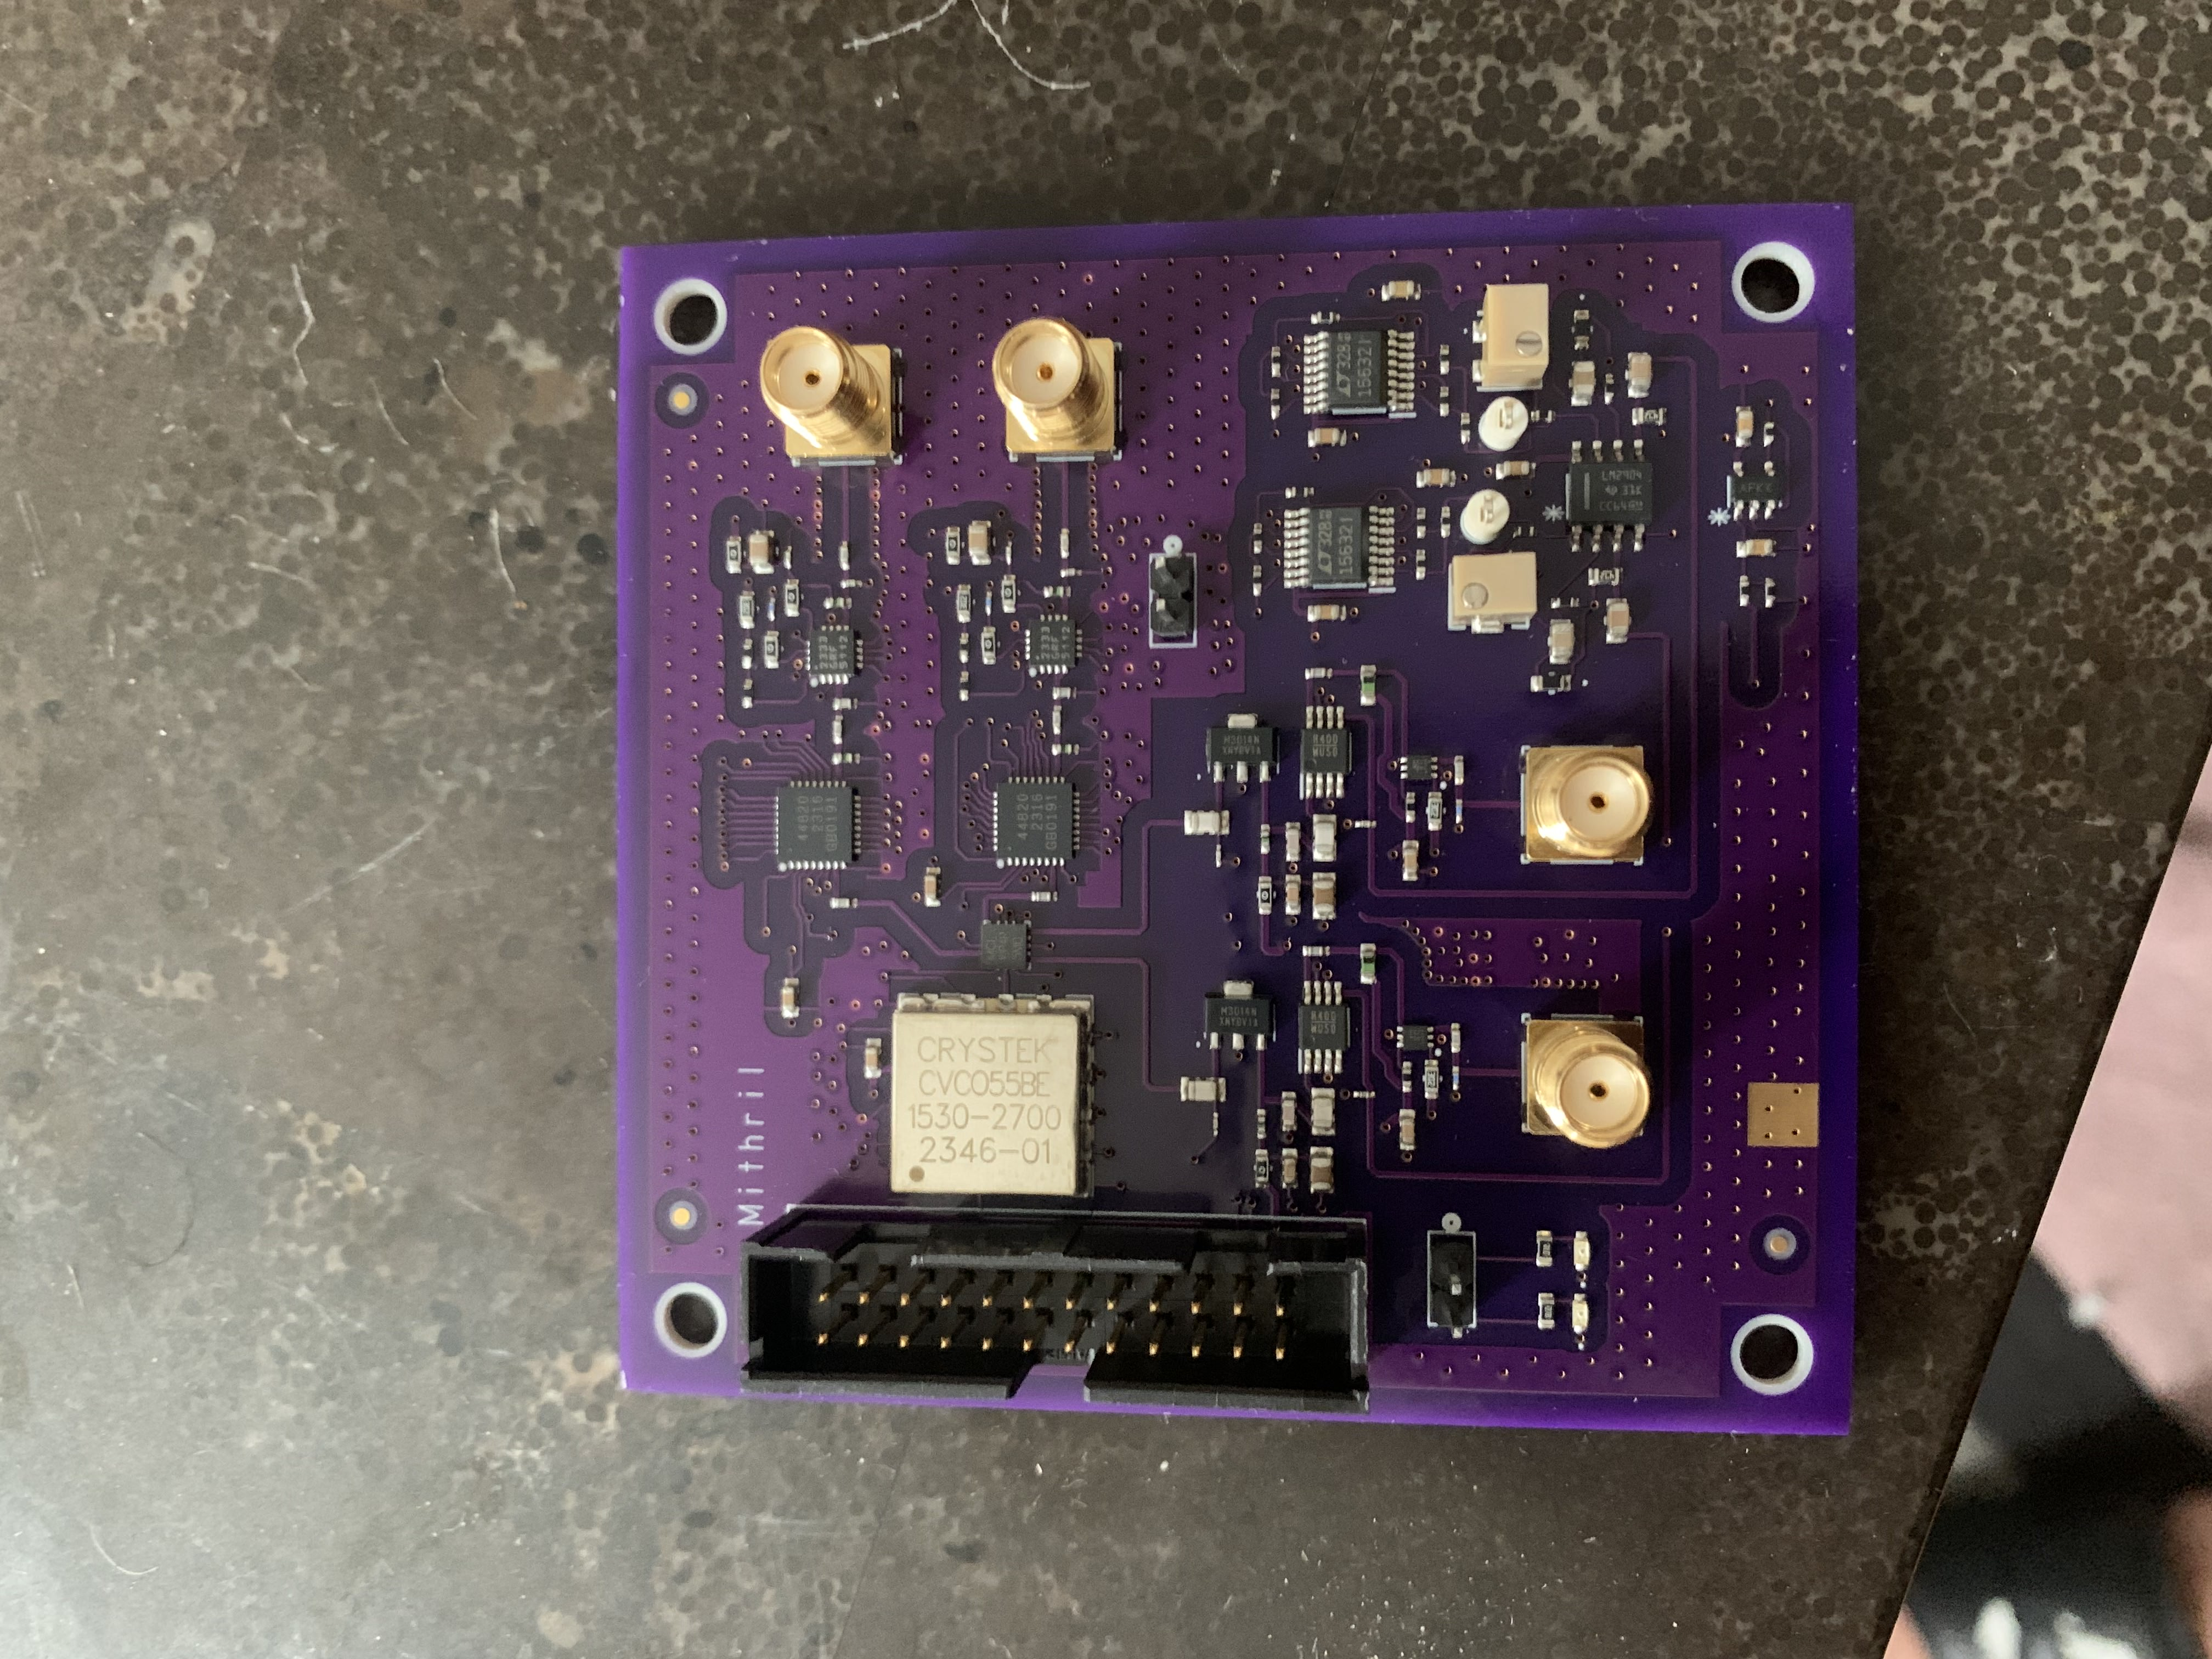
\includegraphics{ProjectImages/pcb_1.jpg}}
\caption{Mithril PCB}
\label{img:mithrilPCB_1}
\end{figure}
The heart of the project is a standalone PCB capable of FMCW radar and phased array beamforming, which can be seen in Image \ref{img:mithrilPCB_1}.
The PCB has a transmitting and receiving portion, each with several stages. The TX portion has a stage for signal synthesis,
phase shifting, and amplification. The RX portion has a stage for amplification, mixing, and baseband filtering/amplifying.
There are also GPIO pins for interfacing with the microcontroller, as well as test pins for analyzing the signals we receive.
This was foreign ground for the entire team, and was started by first researching common RF chains, picking parts that could handle
the afformentioned stages, designing the schematic and layout in ORCad, and then printing and assembling the board. Afterwards,
we tested for weeks to find different issues and workarounds which will be mentioned later.

\section{Digital Processing}
The digital processing was handled entirely by the \href{https://www.st.com/en/evaluation-tools/nucleo-f756zg.html}{STM-F756ZG}.
Two of them were used in the final implementation, where one was responsible for generating a ramp voltage which will be discussed
later, and the other responsible for sampling the radar's received signal, windowing the signal, taking the FFT, transmitting 
the FFT over UART, and receiving commands over UART to program the phase shifter on the PCB via its GPIO pins. This was a lot of tasks,
and all of it was programmed to run in a superloop with the help of DMA and interrupts.

\section{Networking}
How the fuck does a mesh network work borger.



